The main idea behind this project was to use the \textit{Pandaboard} - an embedded development board - to output information on an external device, in this case a LED bar with 40 LED's. The goal was to create the drivers and to be able to use it universally. We wanted to create the possibility to write different applications for this system, without changing anything on the driver level of the \textit{Pandaboard}. 
Examples for so called \textit{User-space} application are measuring the quality of a connected WLAN, measuring the signal strength of a WLAN and also to output the \textit{Load} - CPU usage - of the \textit{Pandaboard}.

\section{Pandaboard}
The \textit{Pandaboard} is a low-power, low-cost single-board computer development platform based on the Texas Instruments OMAP44xx system-on-a-chip family. \footnote{More about the \textit{Pandaboard} can be found on \url{http://pandaboard.org/}  and  \url{http://en.wikipedia.org/wiki/PandaBoard}.} 

\begin{figure}[H]
   \centering
   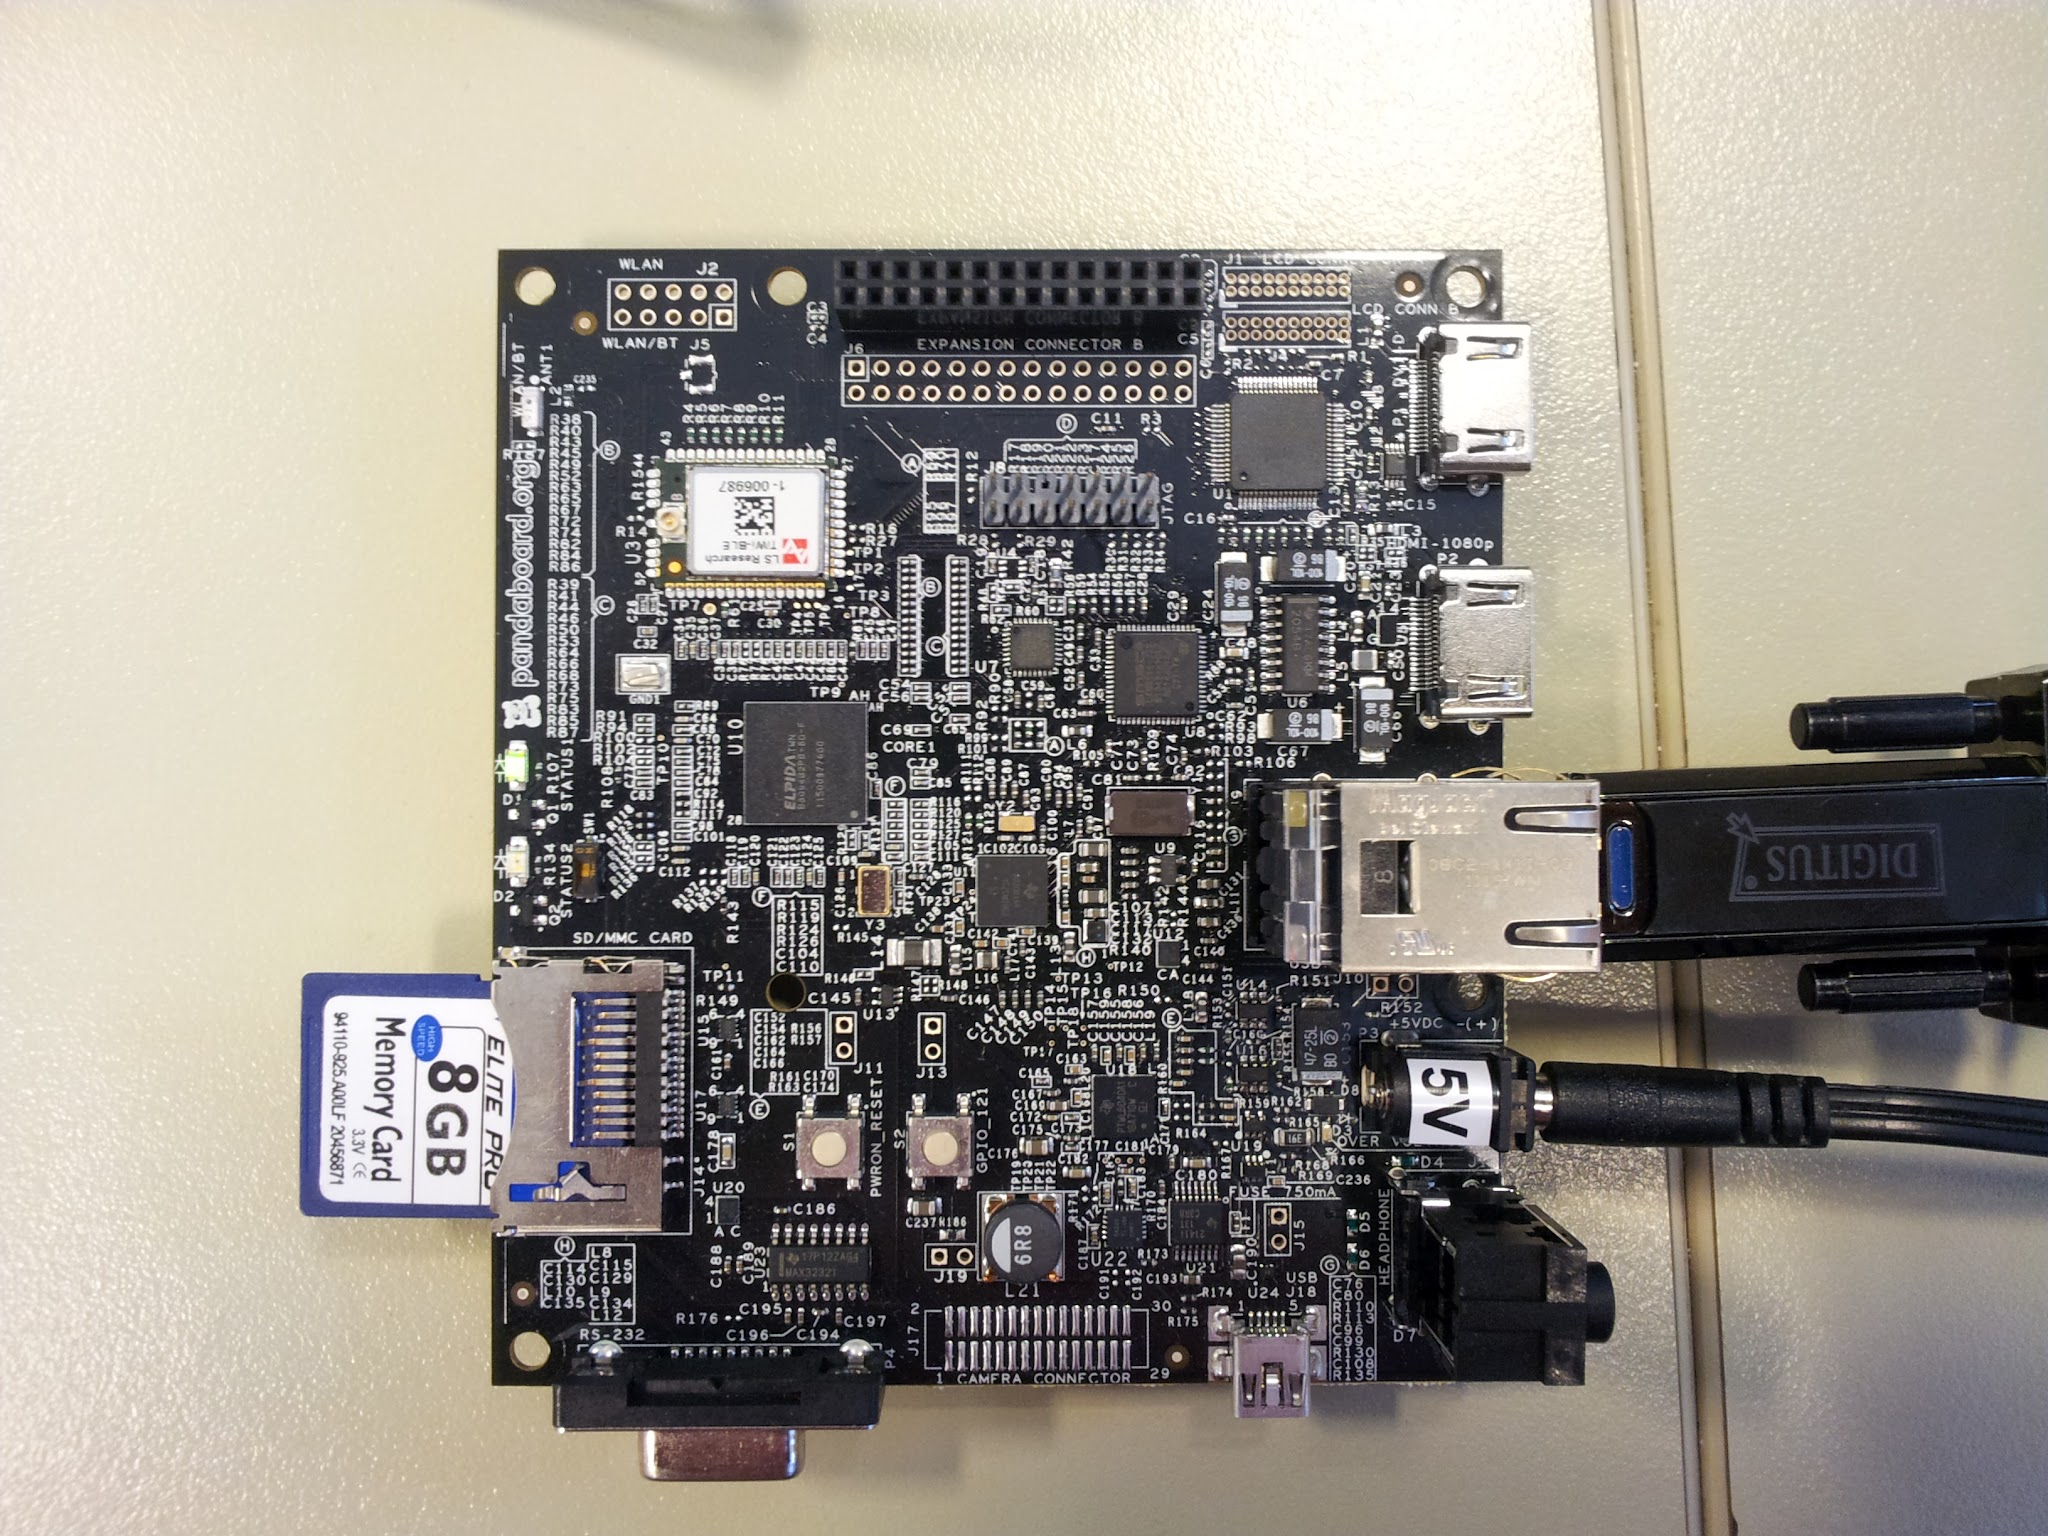
\includegraphics[width=0.8\textwidth]{img/Pandaboard_Alone.jpg}%
   \caption{Pandaboard with installed SD card}
   \label{fig:pandaBoard_Alone}%
\end{figure}

\newpage
\subsection{Features of the Pandaboard}
In the following table we will show the most important hardware features of the \textit{Pandaboard}.

\begin{table}[h]
\centering
\begin{tabular}{| l |  p{7cm} |}
\hline
\textbf{Feature} & \textbf{Specification} \\ \hline
CPU & OMAP4430 dual-core 1 GHz ARM Cortex-A9 MPCore CPU \\ \hline
Memory & 1 GB low power DDR2 RAM \\ \hline
GPU & POWERVR™ SGX540 graphics core supporting all major API's including OpenGL® ES v2.0, OpenGL ES v1.1, OpenVG v1.1 and EGL v1.3 \\ \hline
Audio & Low power audio, 3.5"  Audio in/out \\ \hline
Storage & Full size SD/MMC card cage \\ \hline
LAN & Onboard 10/100 Ethernet \\ \hline
Wireless connections & 802.11 b/g/n, Bluetooth® v2.1 + EDR \\ \hline
Expansiona & General purpose expansion header (I2C, SPI, GPMC, USB, MMC, DSS, ETM) \\
\hline
\end{tabular}
\caption{Pandaboard feature list}
\label{tab:pandaBoardTable}
\end{table}

\section{LED-Bar}
\begin{figure}[H]
   \centering
   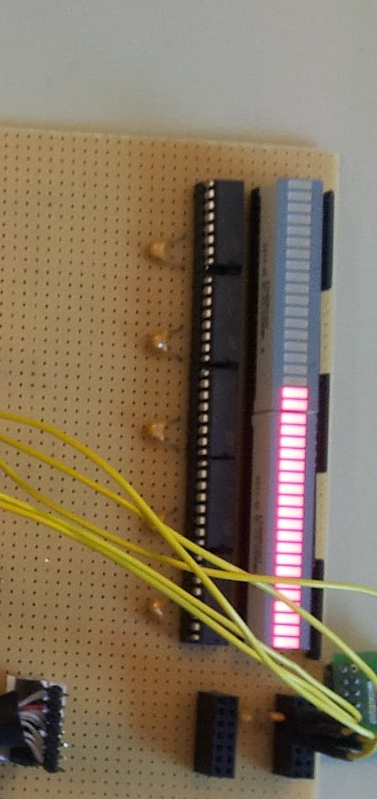
\includegraphics[width=0.3\textwidth]{img/LED-Bar.png}%
   \caption{LED-Bar with 40 LED's and level-shifter.}
   \label{fig:ledBar}%
\end{figure}

\section{Goal to achieve}
\begin{figure}[H]
   \centering
   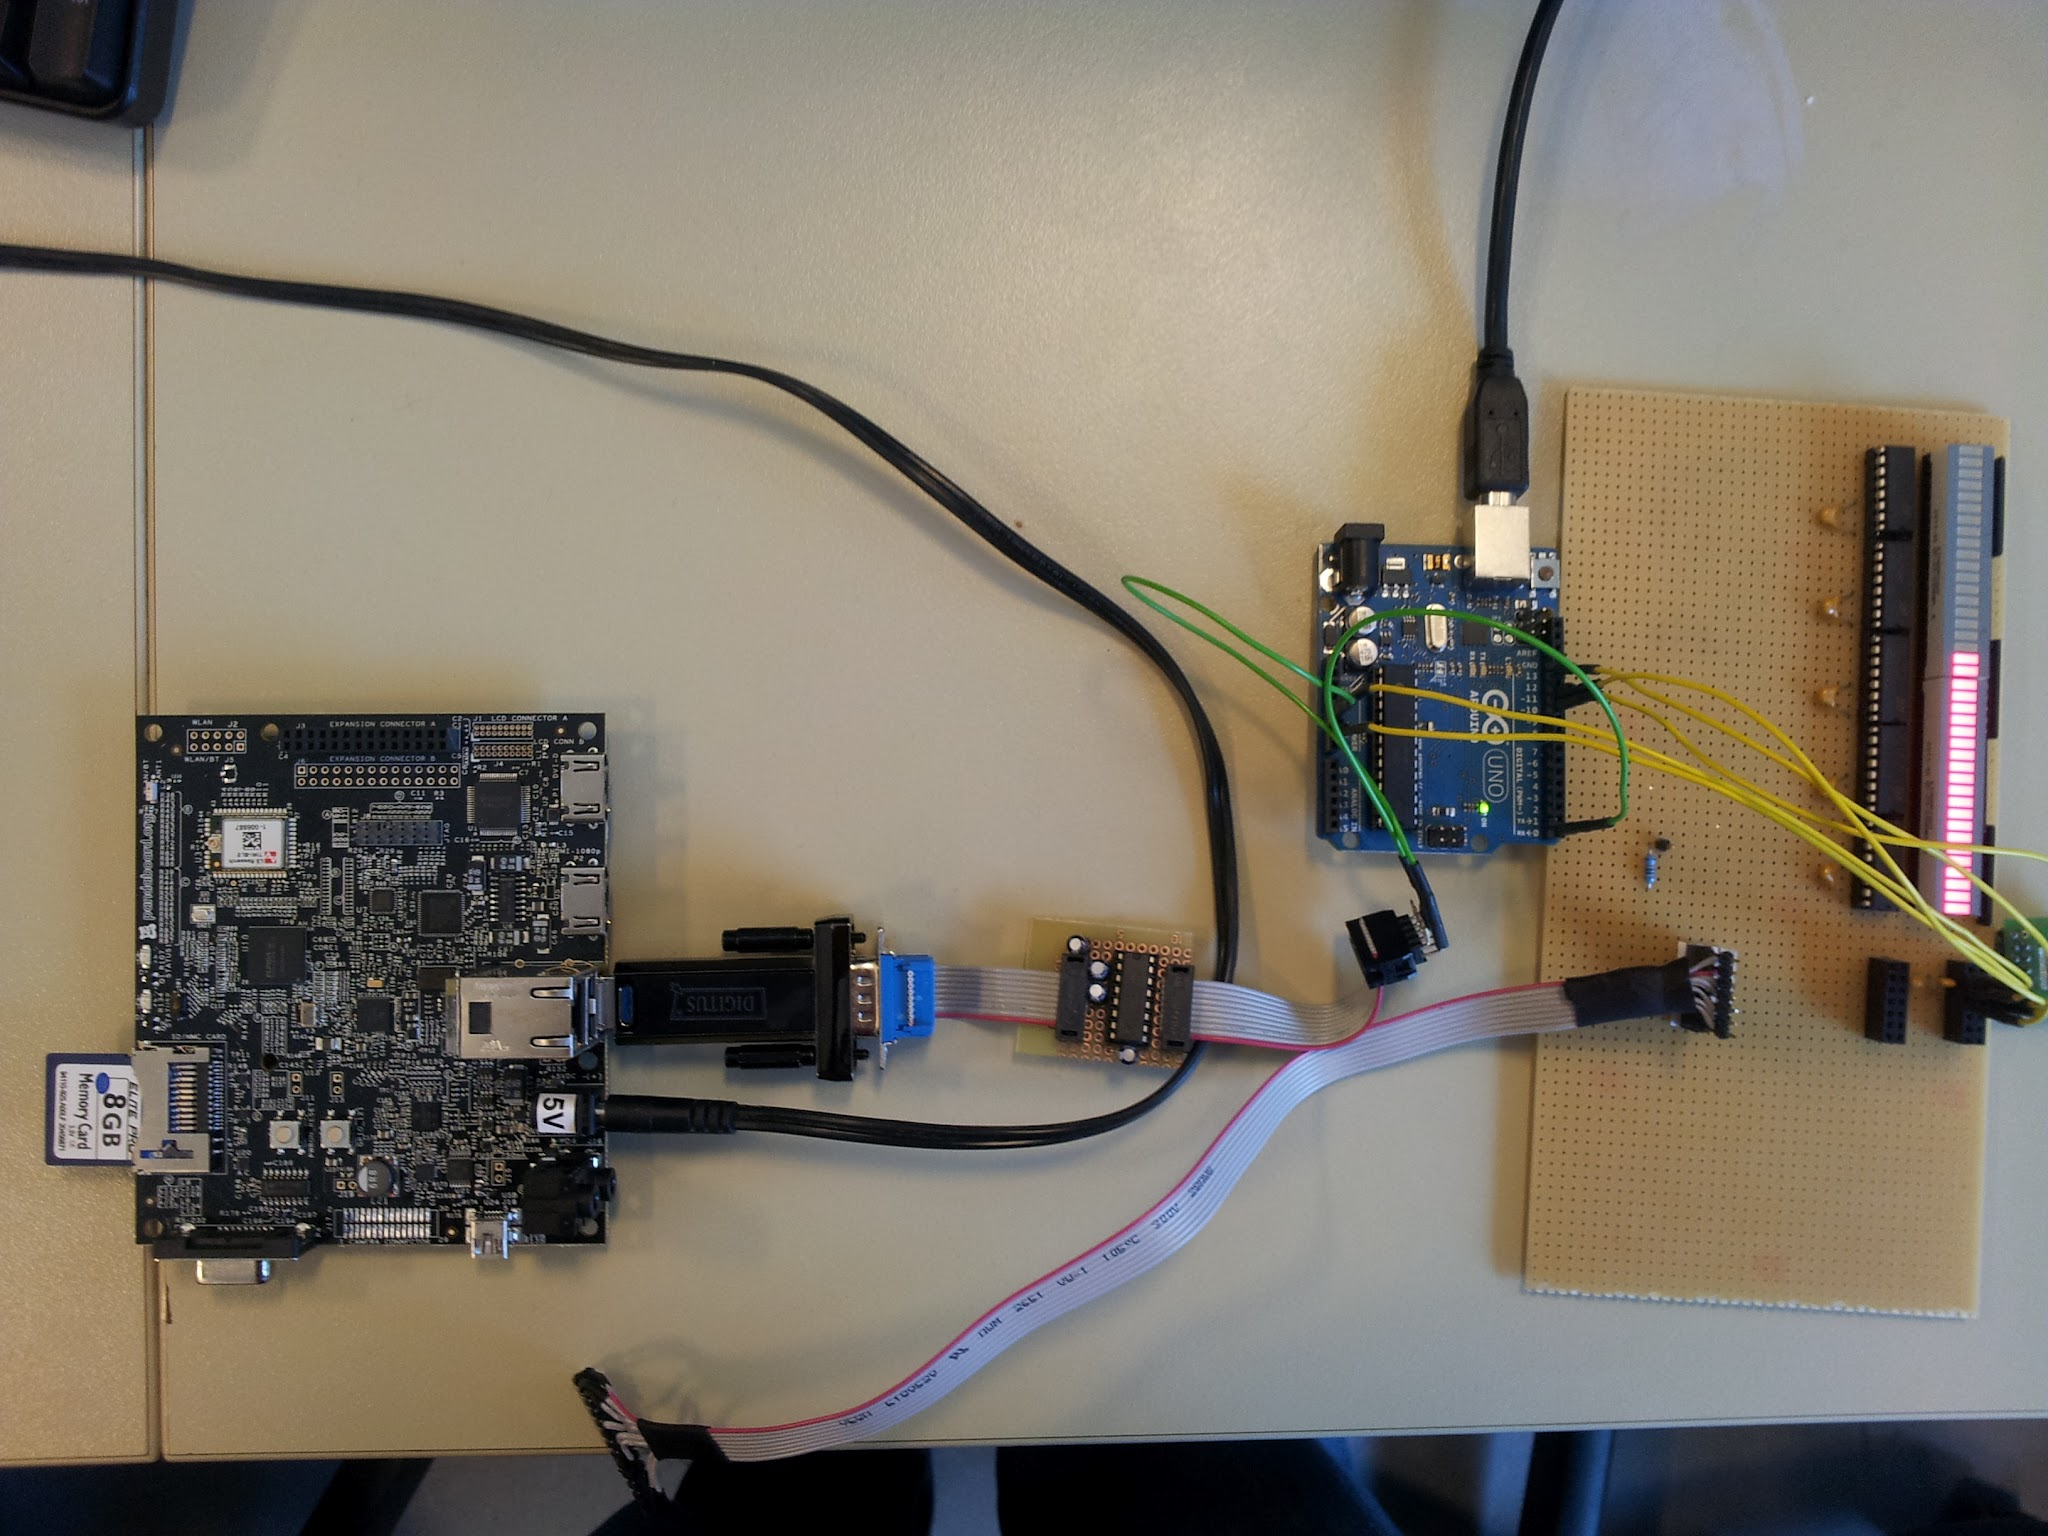
\includegraphics[width=0.8\textwidth]{img/Panda_and_LED_Bar.jpg}%
   \caption{Powering the LED-bar with the Pandaboard and a microcontroller}
   \label{fig:completeProject}%
\end{figure}